\subsection{Algoritmos de Ordenamiento}
El análisis experimental expone una fuerte sensibilidad a la distribución inicial de los datos.

\begin{figure}[H]
    \centering
    \begin{minipage}{0.48\textwidth}
        \centering
        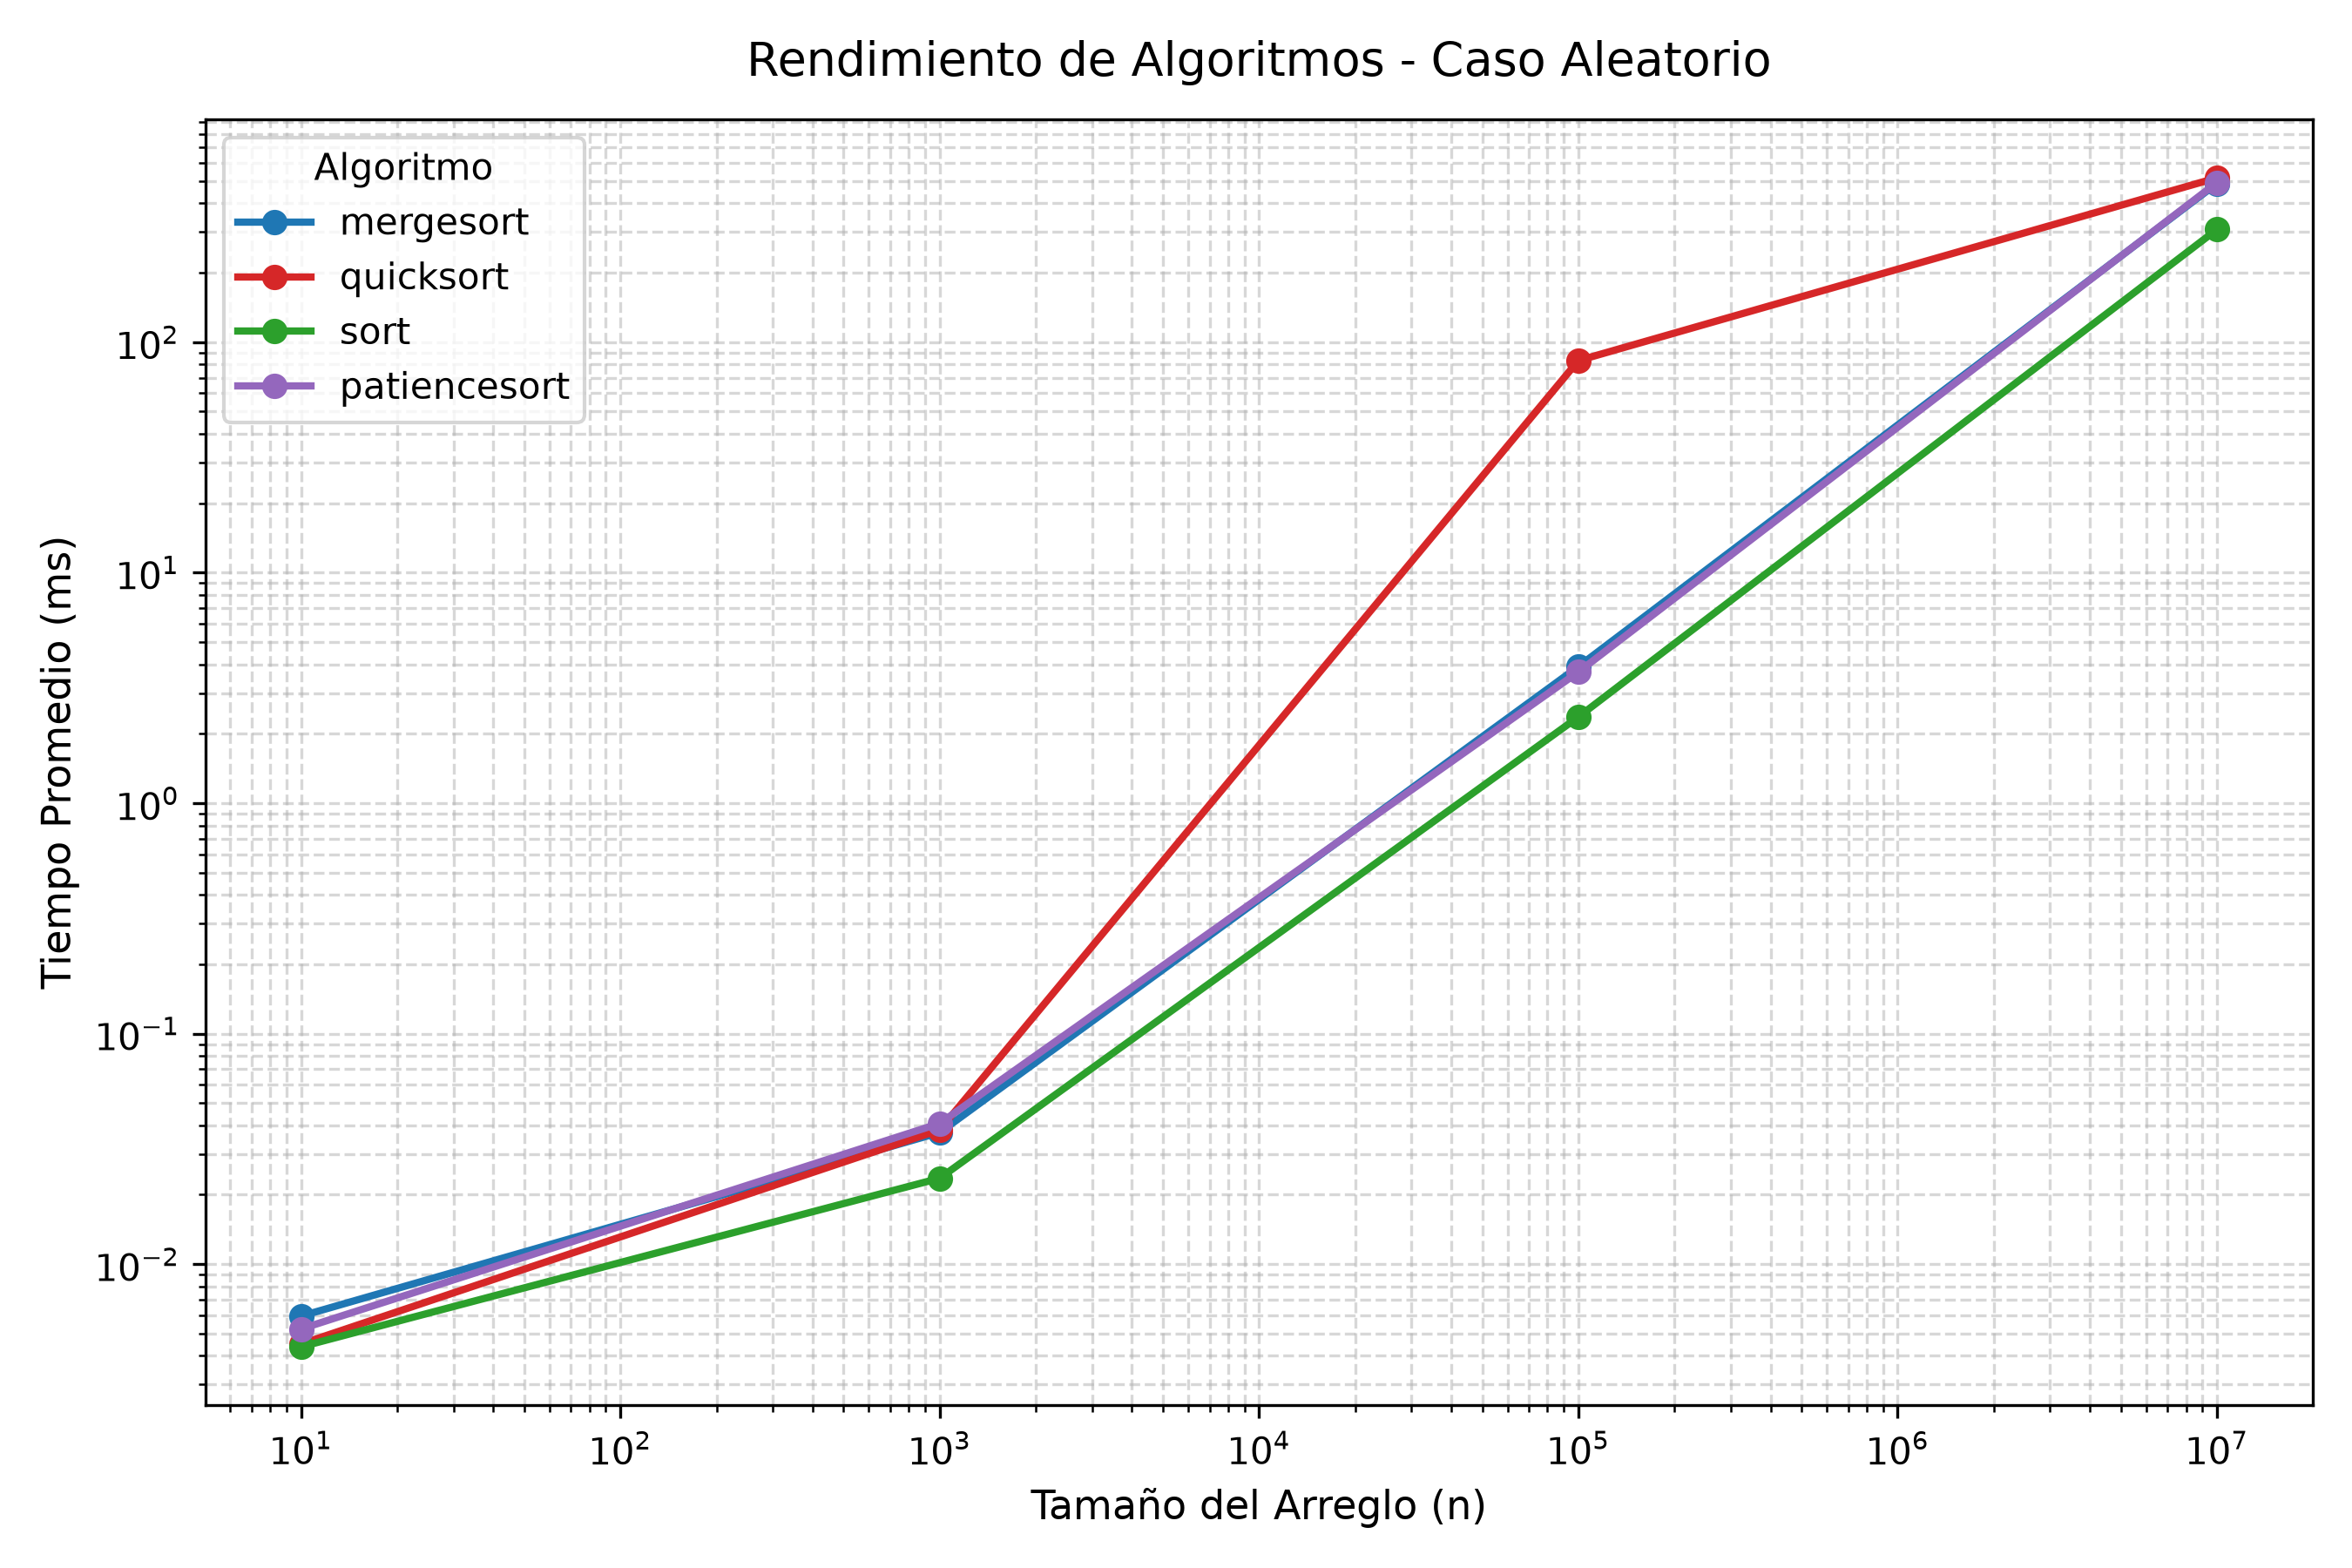
\includegraphics[width=\textwidth]{figures/comparativa_aleatorio.png}
        \caption{Tiempo: Caso aleatorio.}
        \label{fig:t_aleatorio}
    \end{minipage}\hfill
    \begin{minipage}{0.48\textwidth}
        \centering
        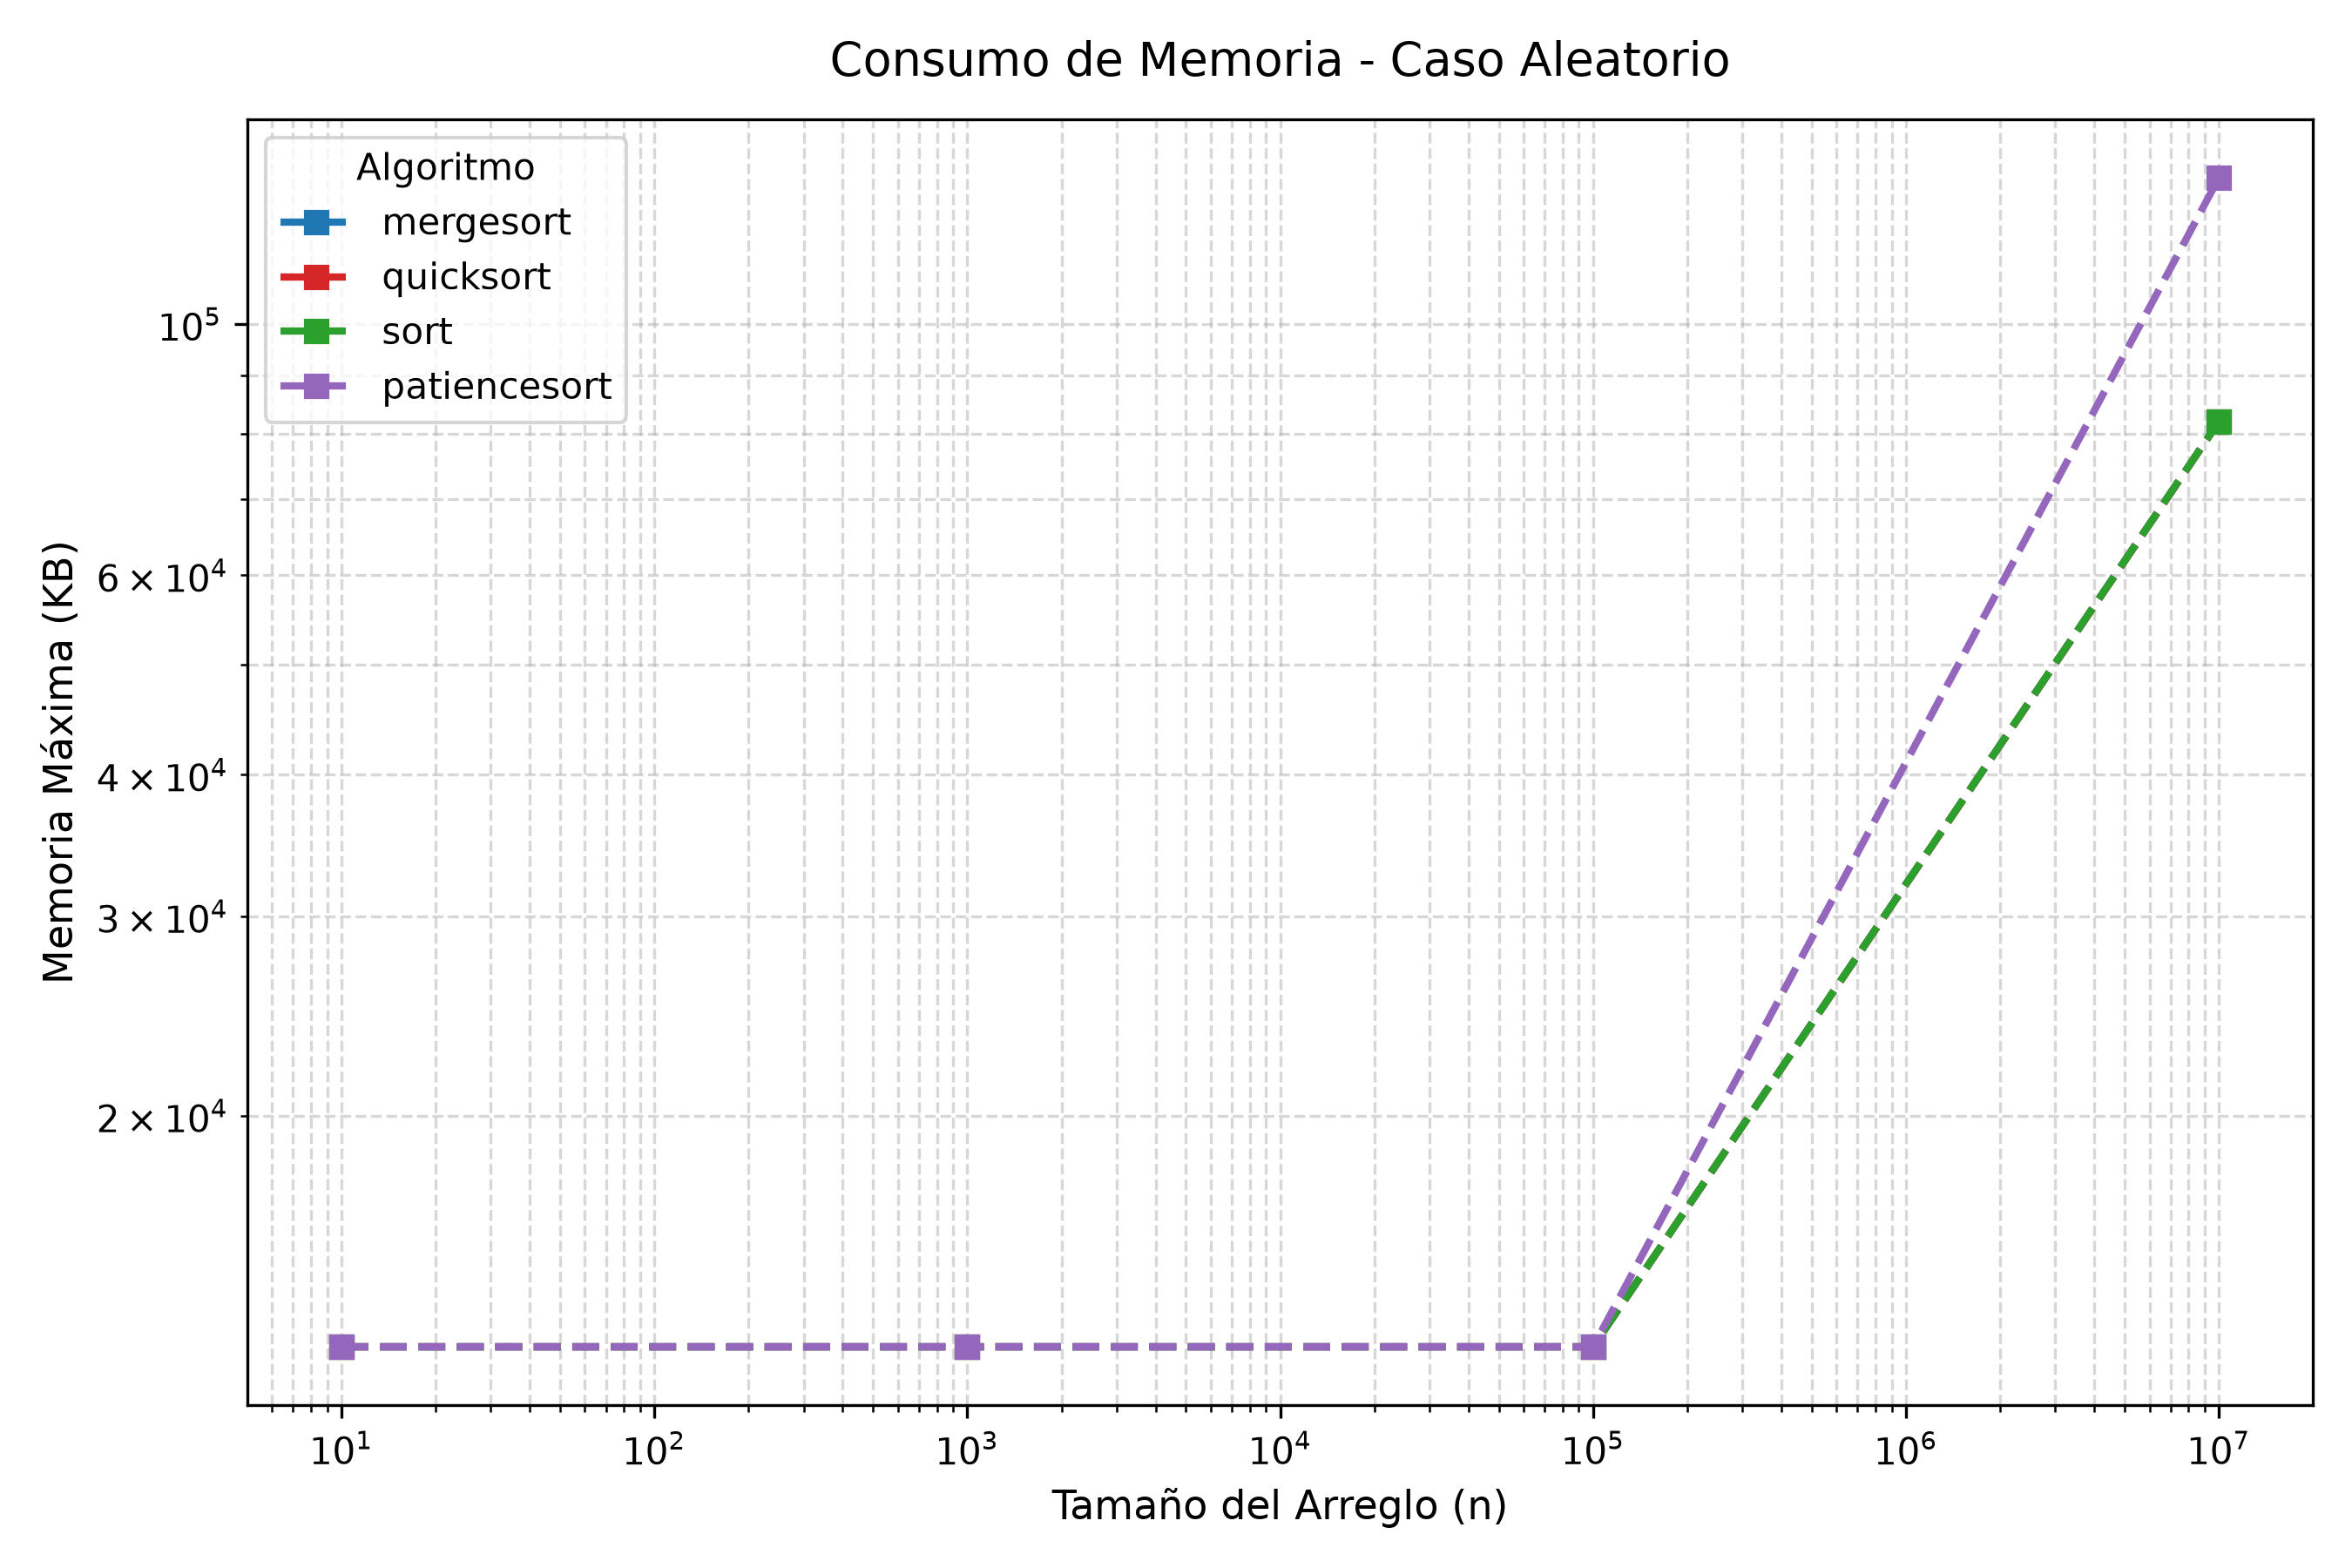
\includegraphics[width=\textwidth]{figures/memoria_aleatorio.png}
        \caption{Memoria: Caso aleatorio.}
        \label{fig:m_aleatorio}
    \end{minipage}
\end{figure}

En la Figura \ref{fig:t_aleatorio}, \texttt{std::sort} logra la menor latencia. QuickSort sufre una degradación catastrófica a $\mathcal{O}(N^2)$ con arreglos ordenados, consumiendo toda la pila (\textit{Stack Overflow}) o excediendo el límite de tiempo para $N \ge 10^6$. MergeSort conserva su tasa teórica $\mathcal{O}(N \log N)$, mientras que PatienceSort mantiene su cota pero con una alta constante multiplicativa. Respecto a la memoria (Figura \ref{fig:m_aleatorio}), \texttt{std::sort} domina operando \textit{in-place}, mientras MergeSort y PatienceSort exhiben un crecimiento $\mathcal{O}(N)$ por sus estructuras auxiliares.

\begin{figure}[H]
    \centering
    \begin{minipage}{0.32\textwidth}
        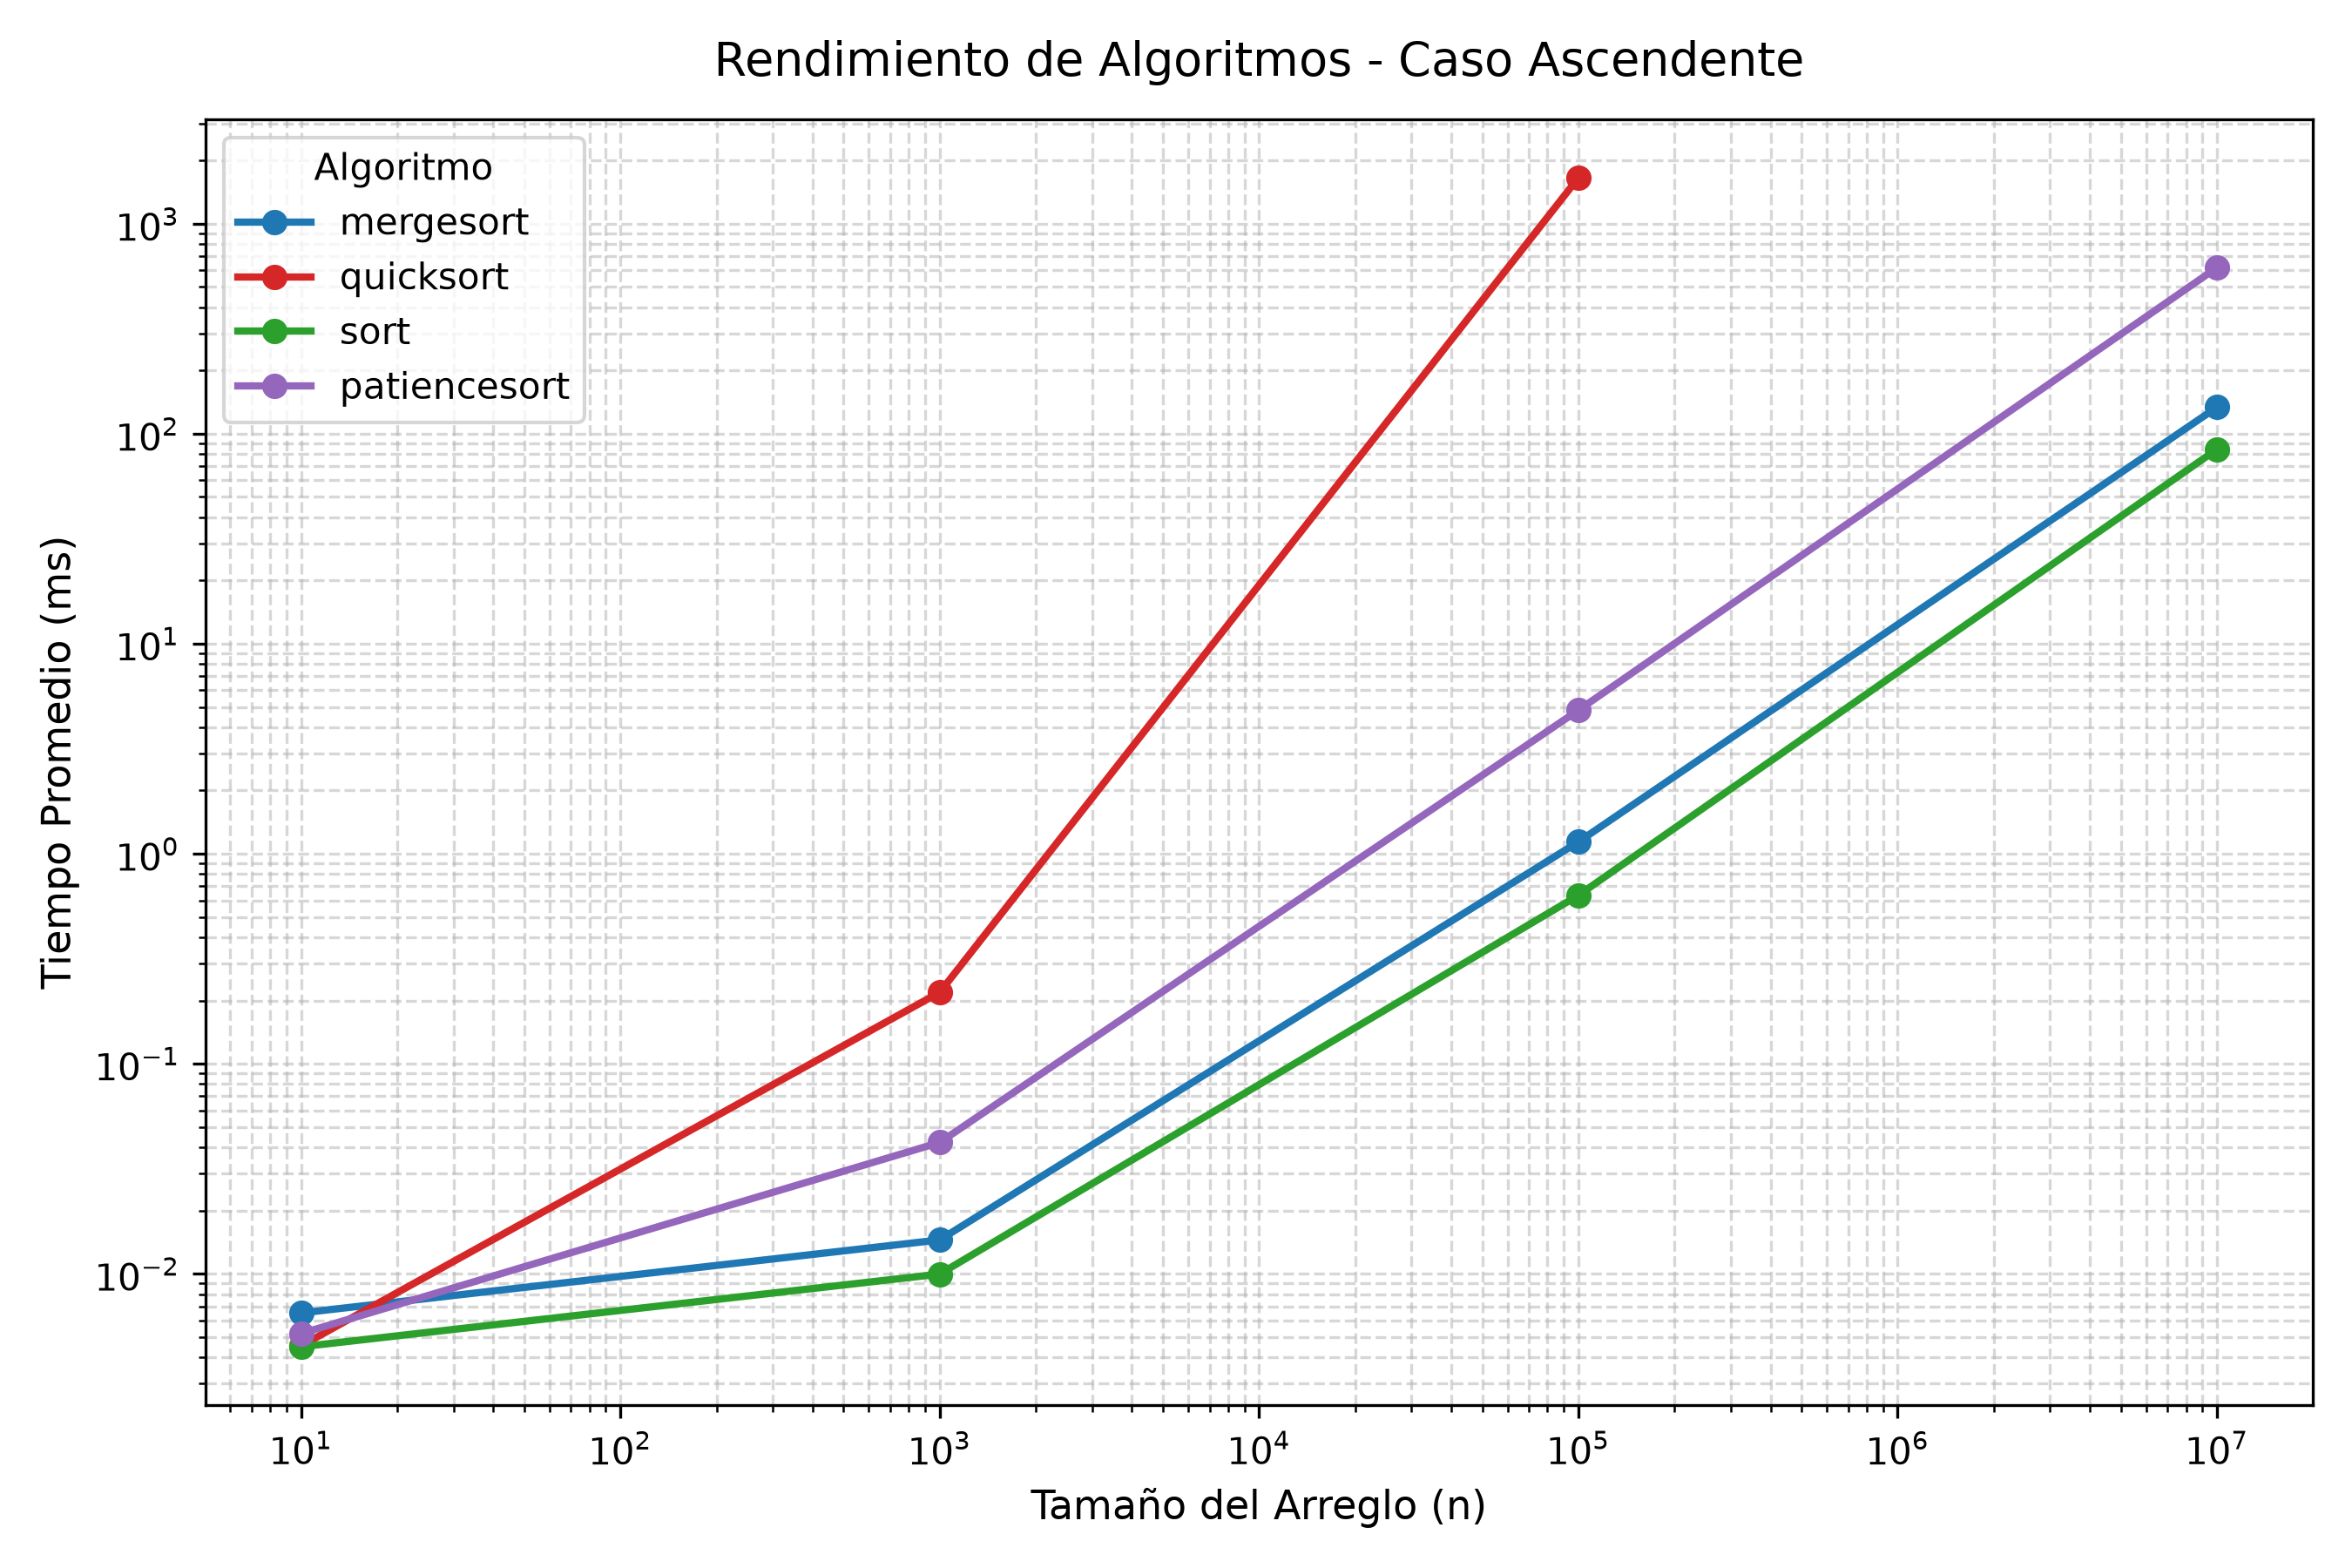
\includegraphics[width=\textwidth]{figures/comparativa_ascendente.png}
        \caption{Ascendente.}
    \end{minipage}\hfill
    \begin{minipage}{0.32\textwidth}
        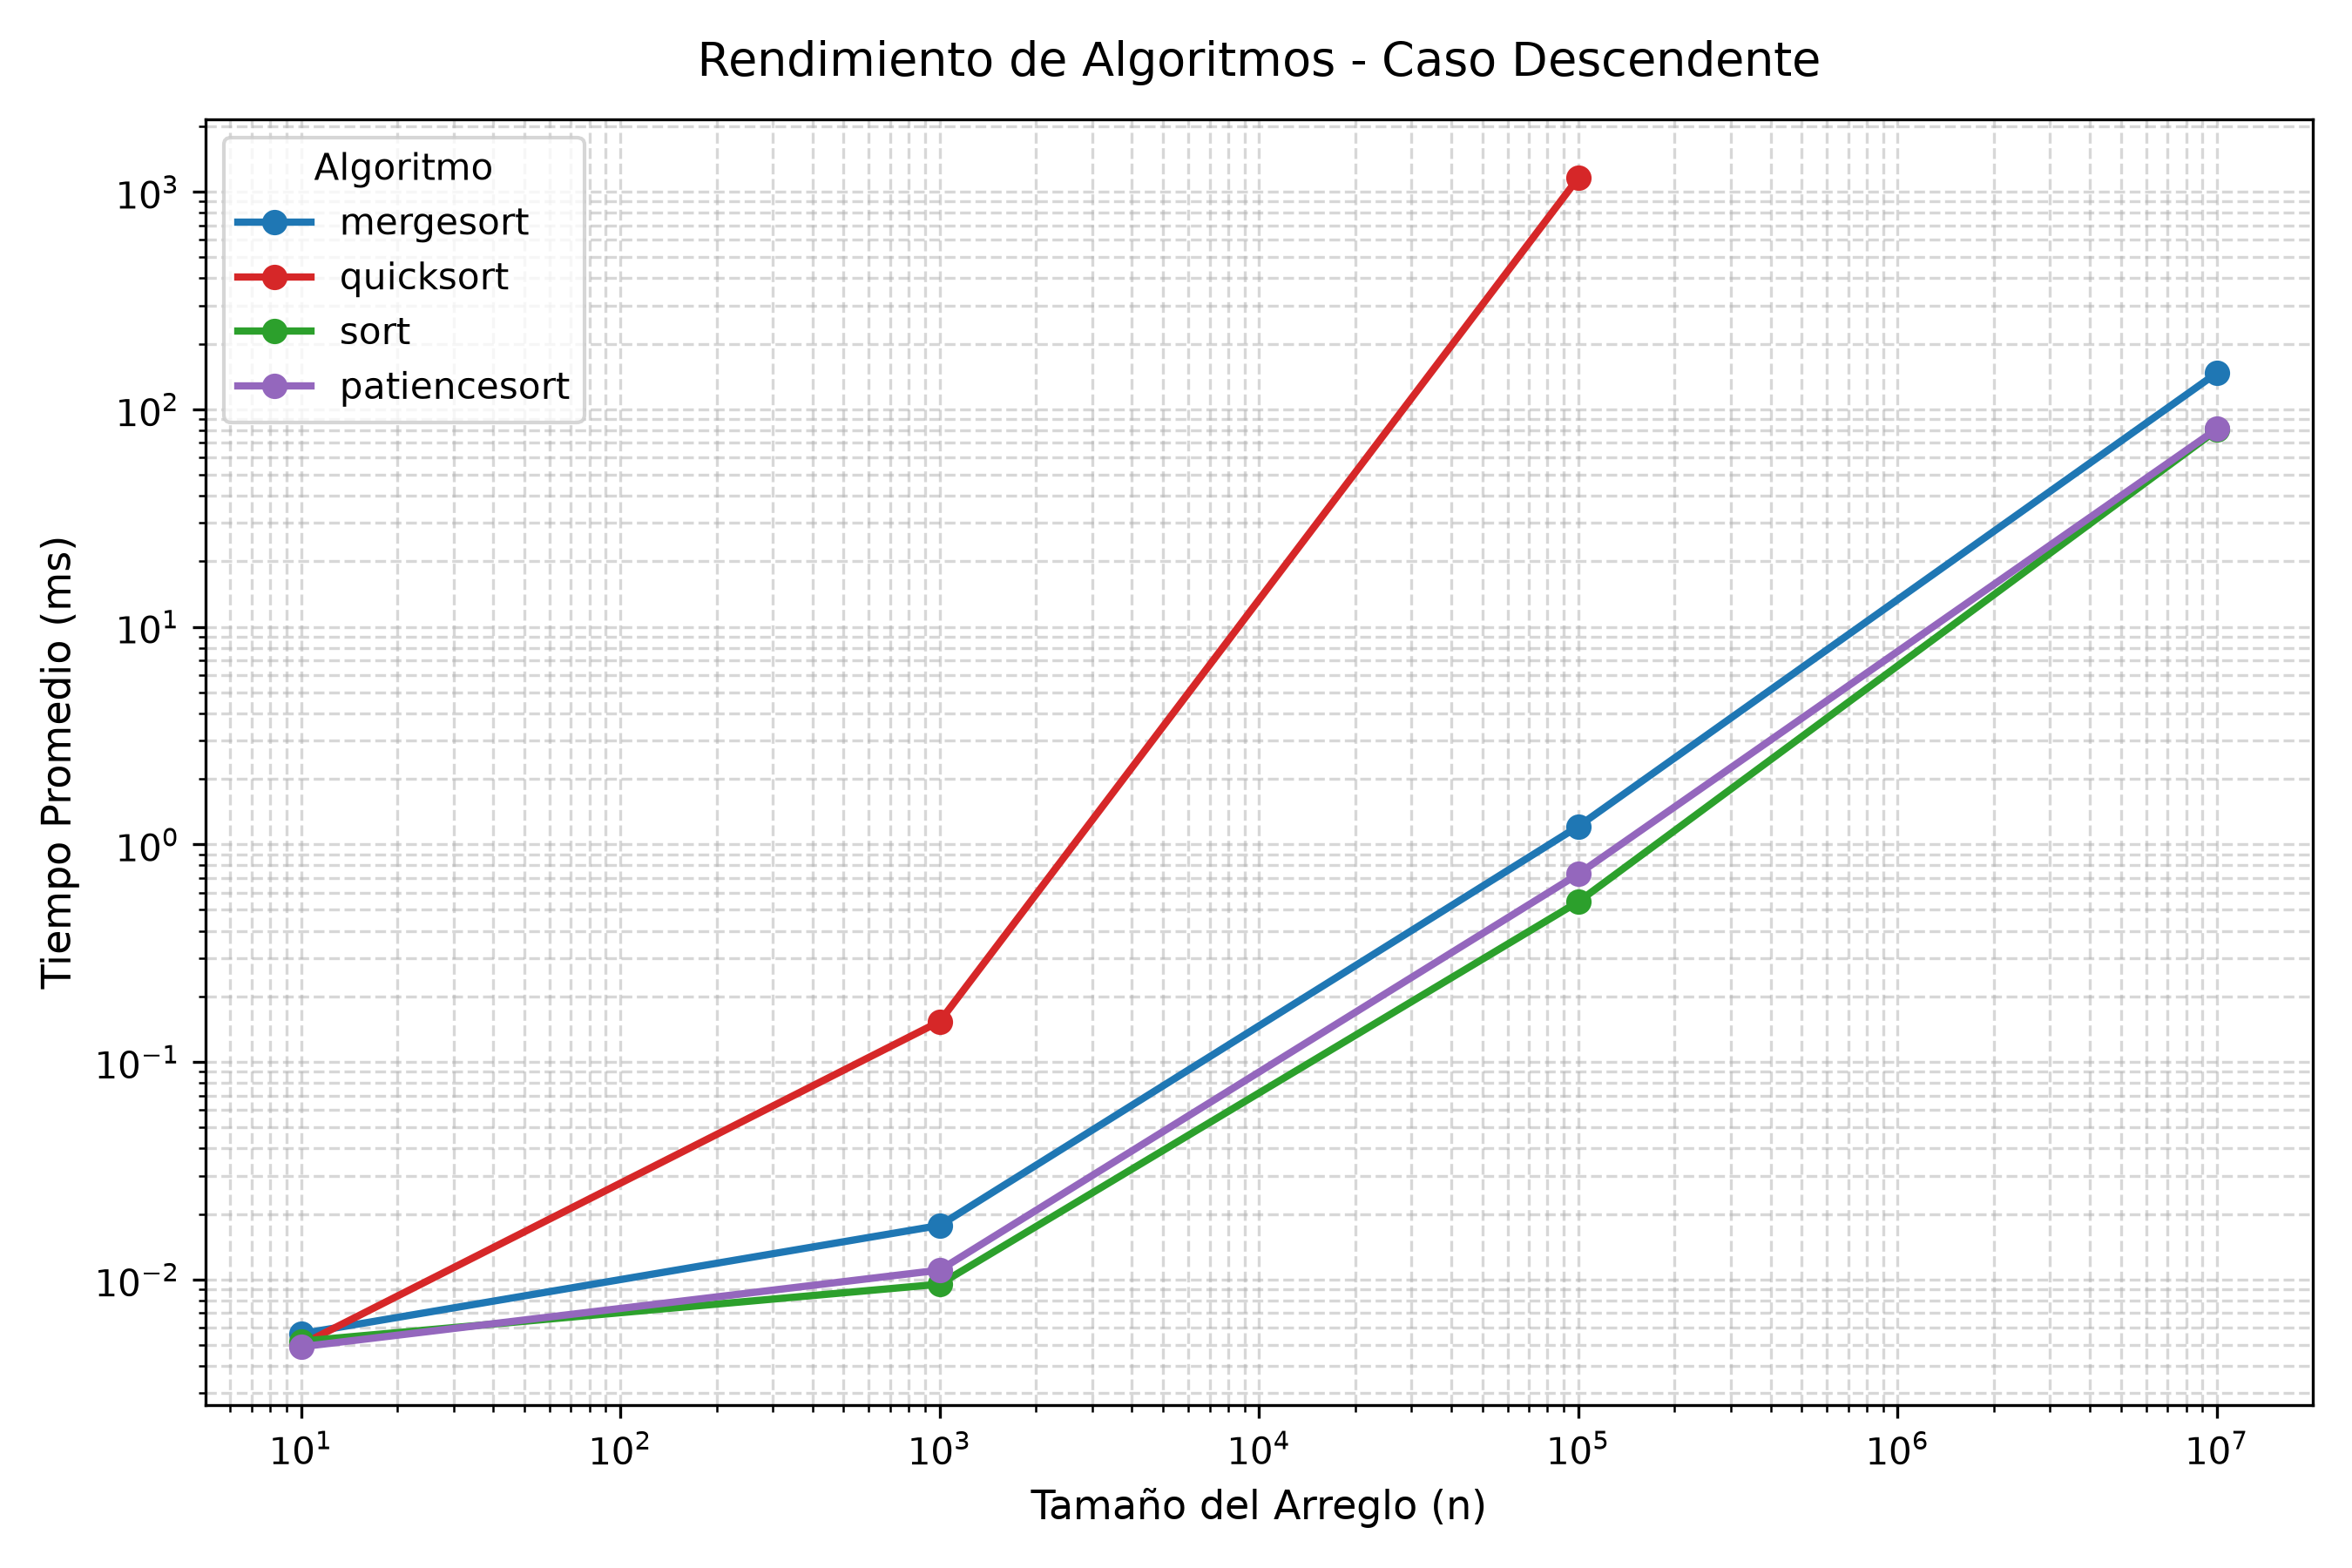
\includegraphics[width=\textwidth]{figures/comparativa_descendente.png}
        \caption{Descendente.}
    \end{minipage}\hfill
    \begin{minipage}{0.32\textwidth}
        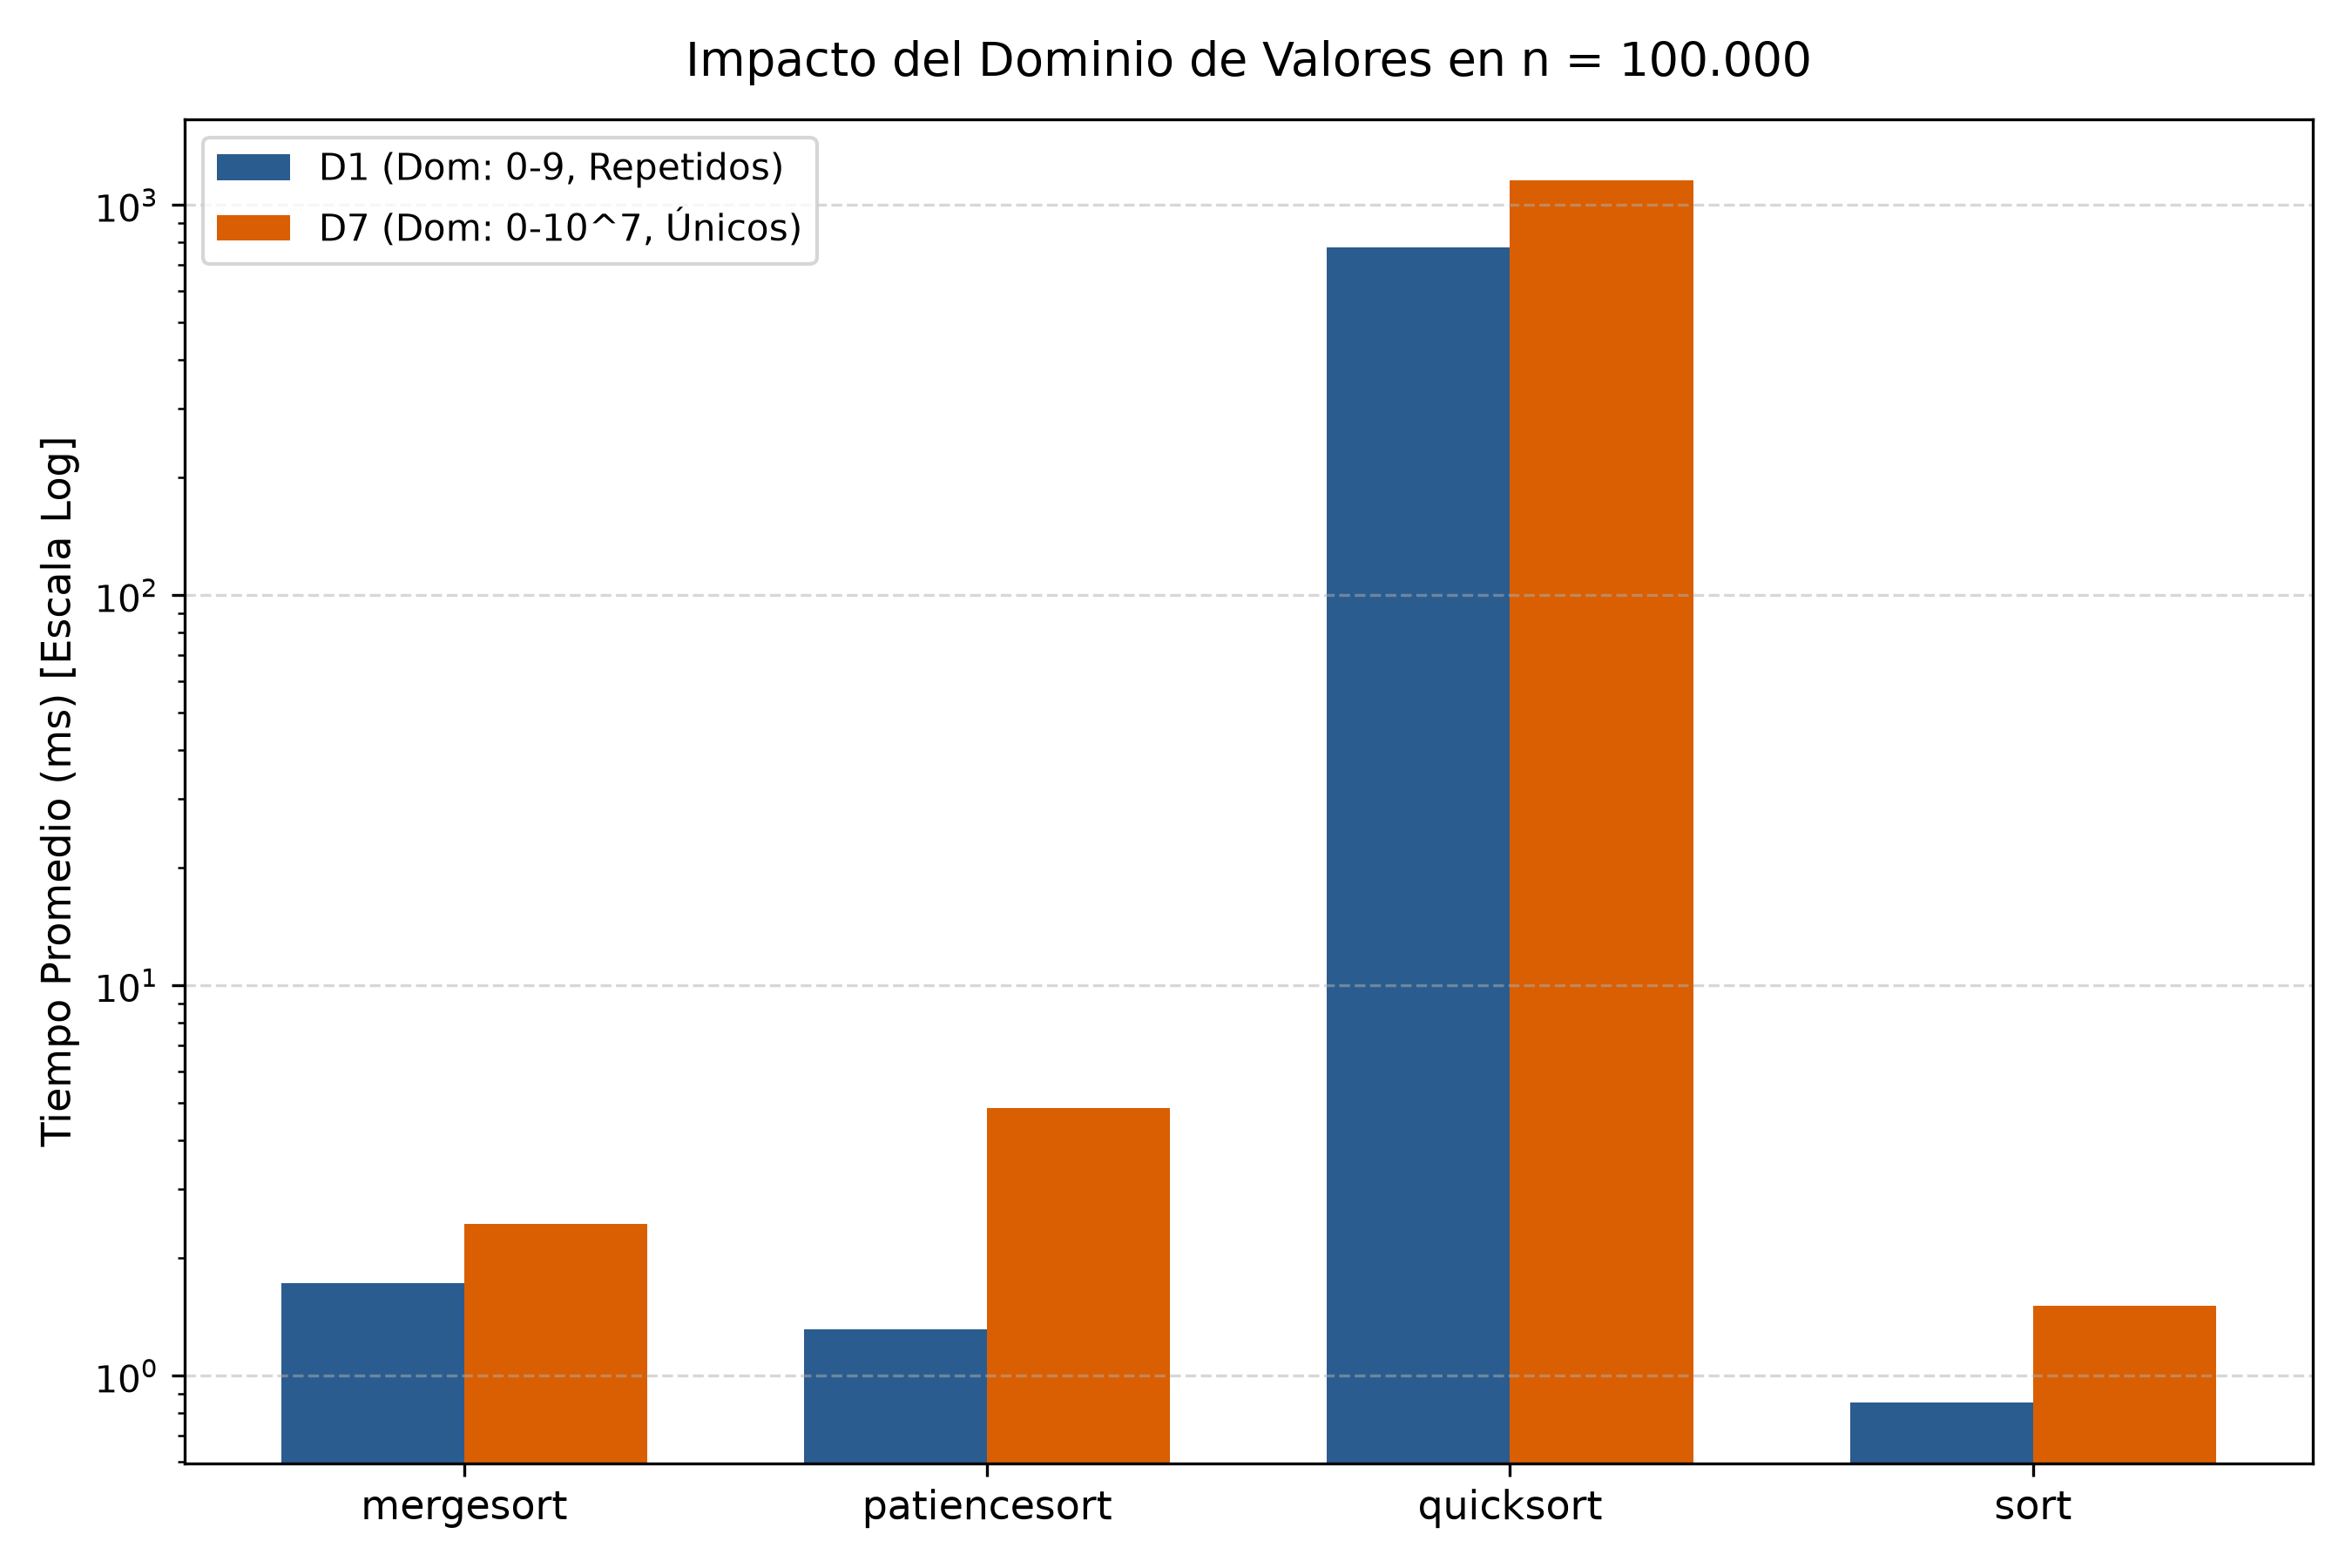
\includegraphics[width=\textwidth]{figures/comparativa_dominios_n100k.png}
        \caption{Dominio ($10^5$).}
    \end{minipage}
\end{figure}

\subsection{Multiplicación de Matrices}

\begin{figure}[H]
    \centering
    \begin{minipage}{0.48\textwidth}
        \centering
        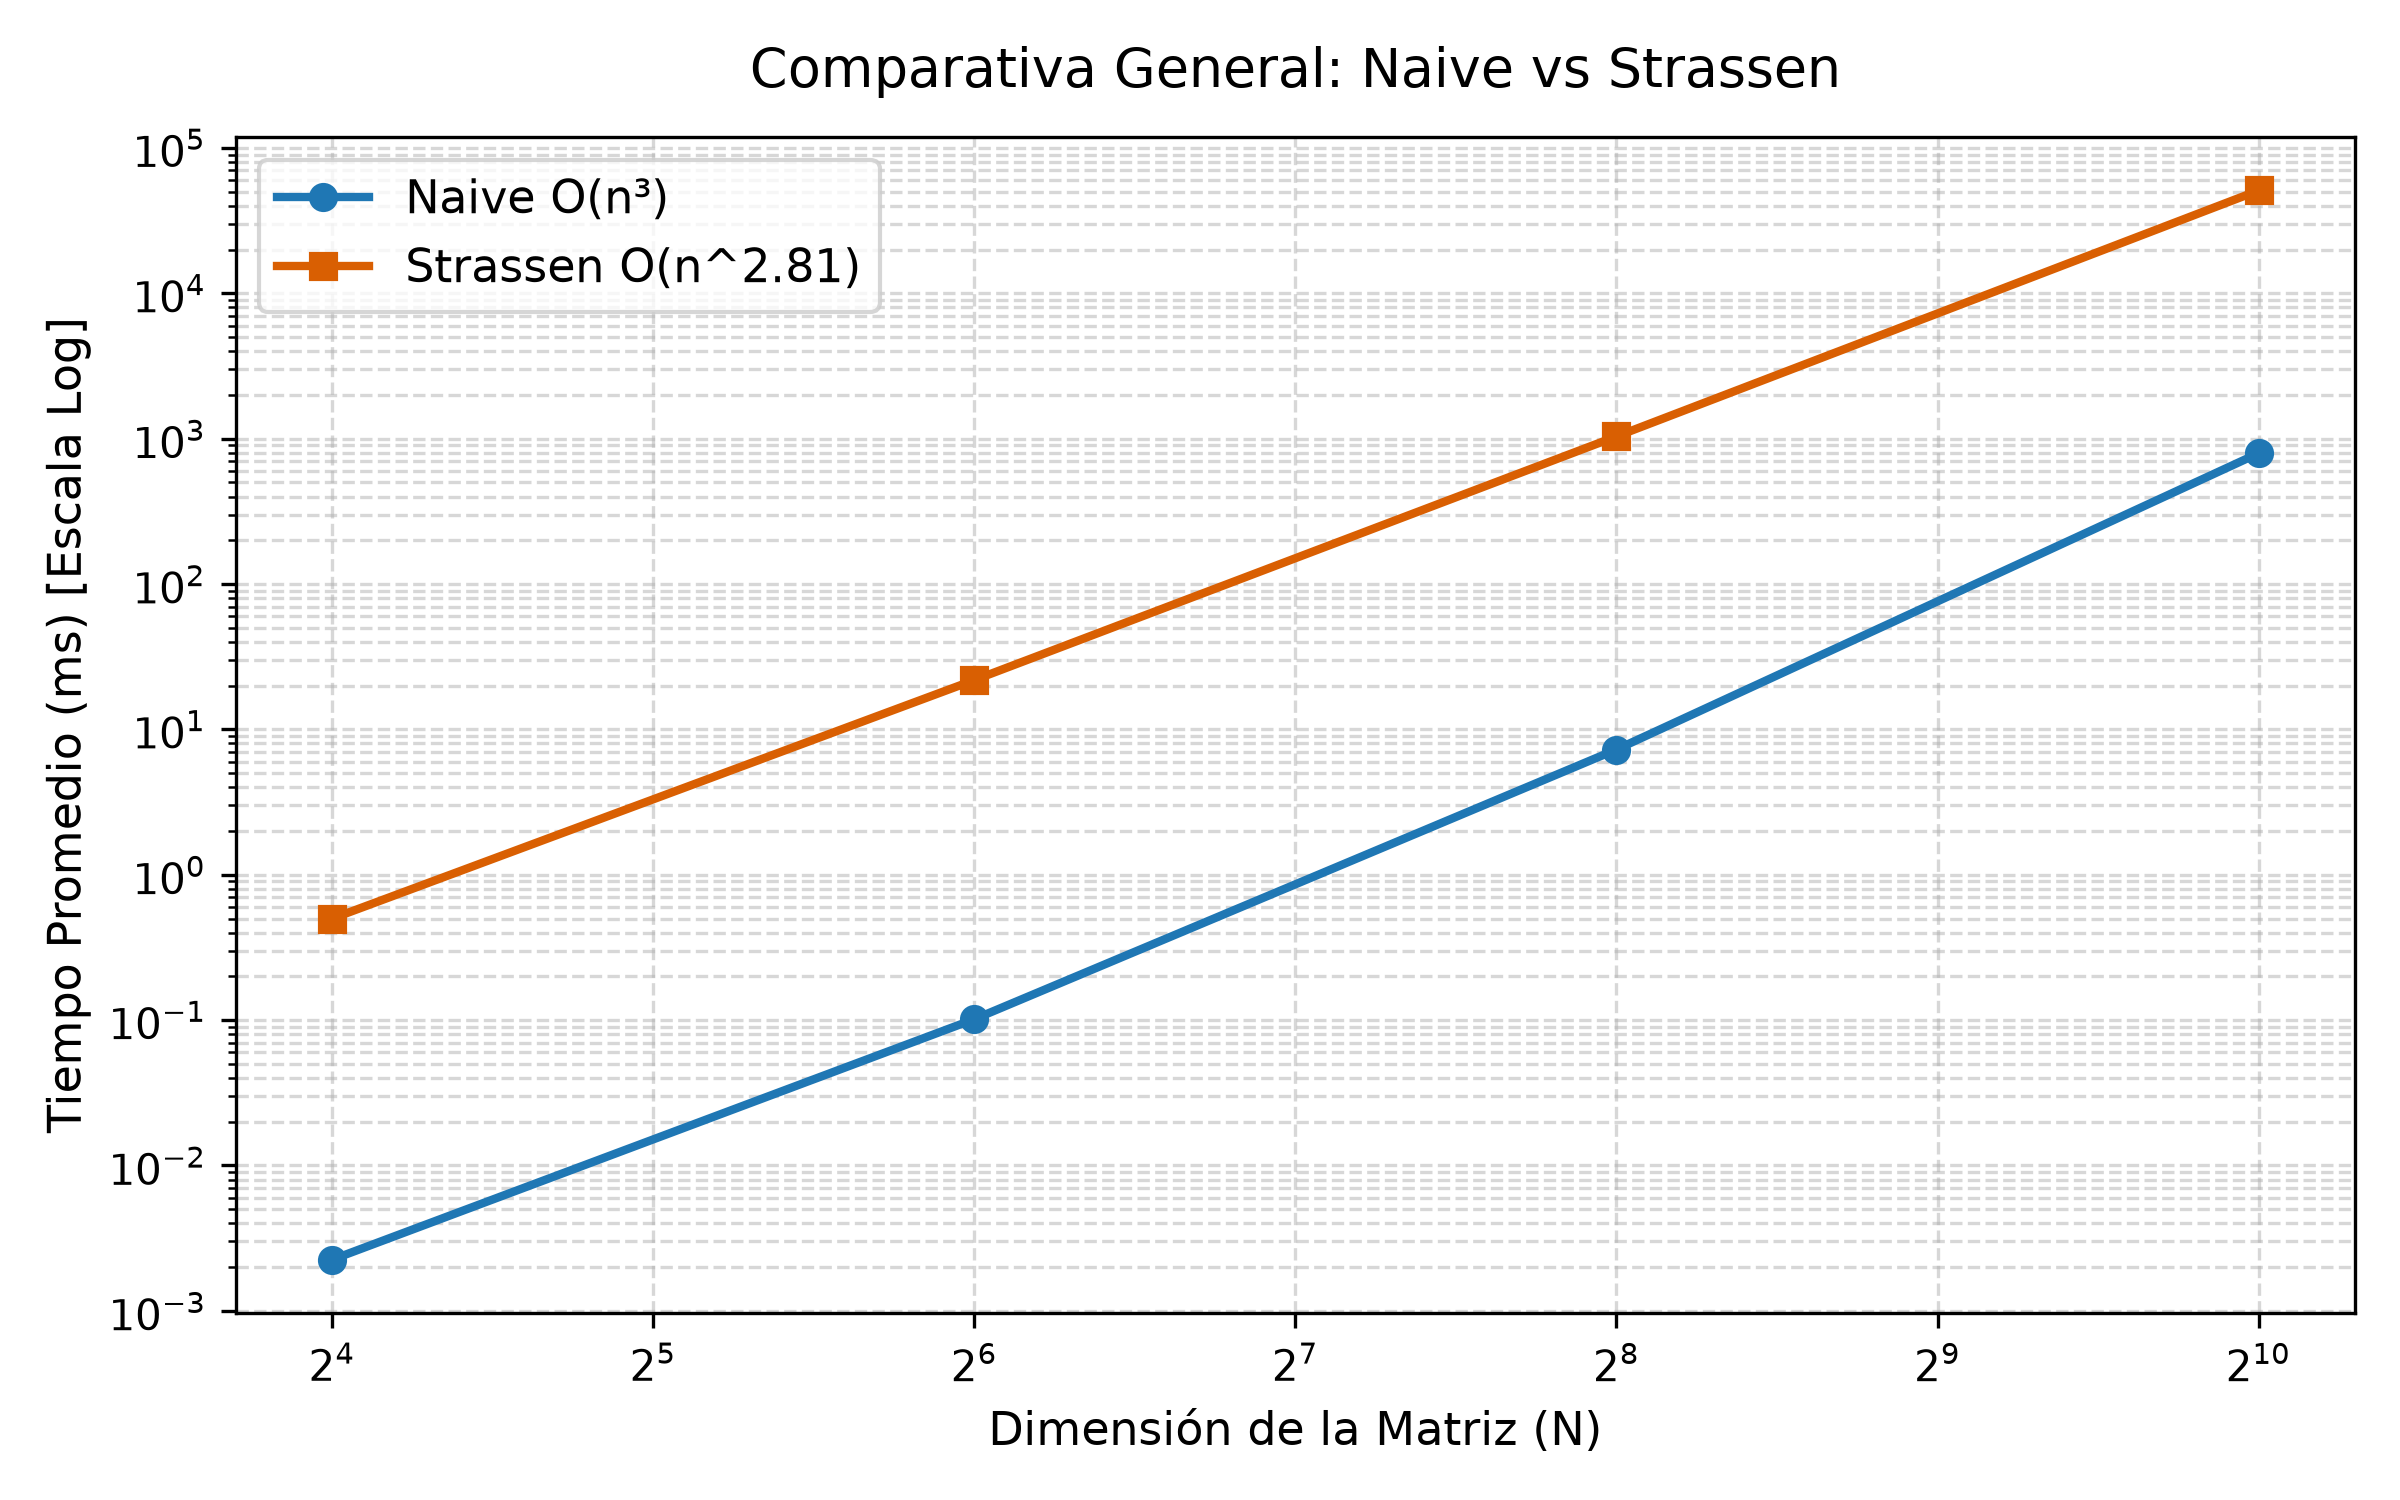
\includegraphics[width=\textwidth]{figures/comparativa_global_matrices.png}
        \caption{Tiempo: Naive vs Strassen.}
        \label{fig:t_matrices}
    \end{minipage}\hfill
    \begin{minipage}{0.48\textwidth}
        \centering
        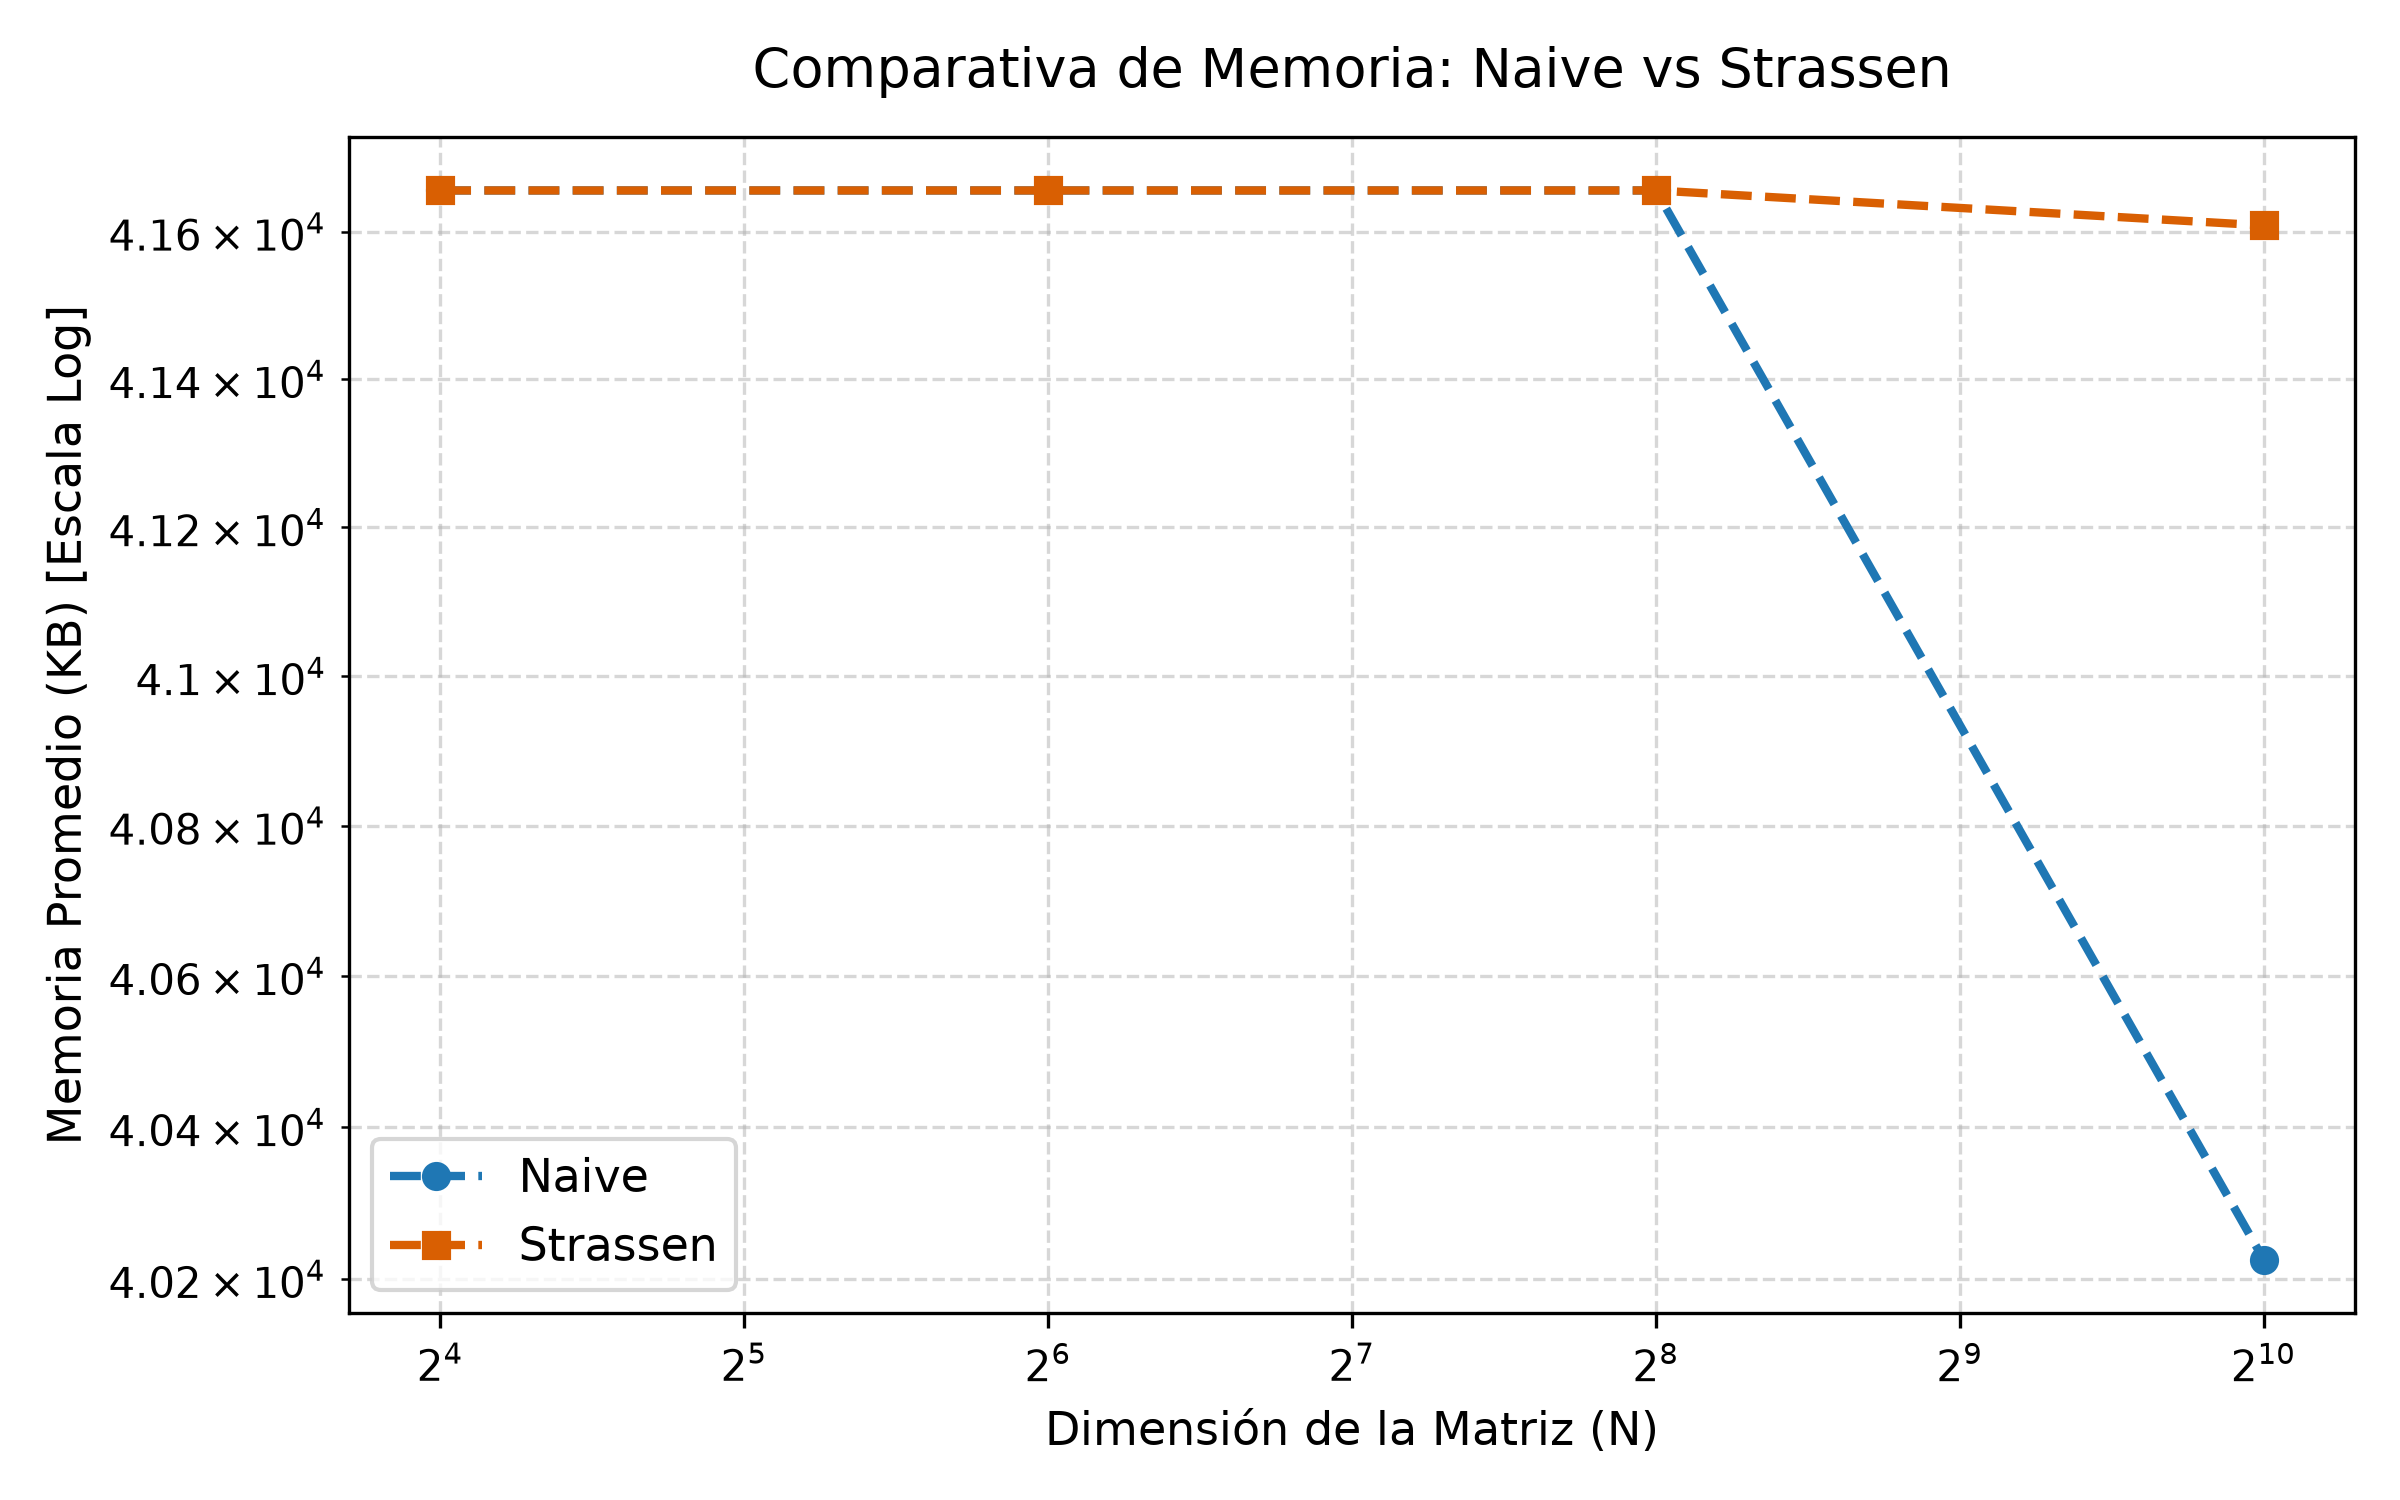
\includegraphics[width=\textwidth]{figures/memoria_global_matrices.png}
        \caption{Memoria: Naive vs Strassen.}
        \label{fig:m_matrices}
    \end{minipage}
\end{figure}

Naive supera por órdenes de magnitud a Strassen (Figura \ref{fig:t_matrices}). La recursividad profunda en $N=1024$ genera $\approx 3.29 \times 10^8$ llamadas, asfixiando la ganancia asintótica por el inmenso \textit{overhead}. Esto se refleja en la Figura \ref{fig:m_matrices}: Strassen exige una asignación masiva en el \textit{heap}, mientras Naive mantiene una huella estable $\mathcal{O}(N^2)$. El tiempo demostró ser agnóstico a la estructura y dominio de las matrices, ya que ninguna implementación omite cálculos sobre ceros.

\begin{figure}[H]
    \centering
    \begin{minipage}{0.48\textwidth}
        \centering
        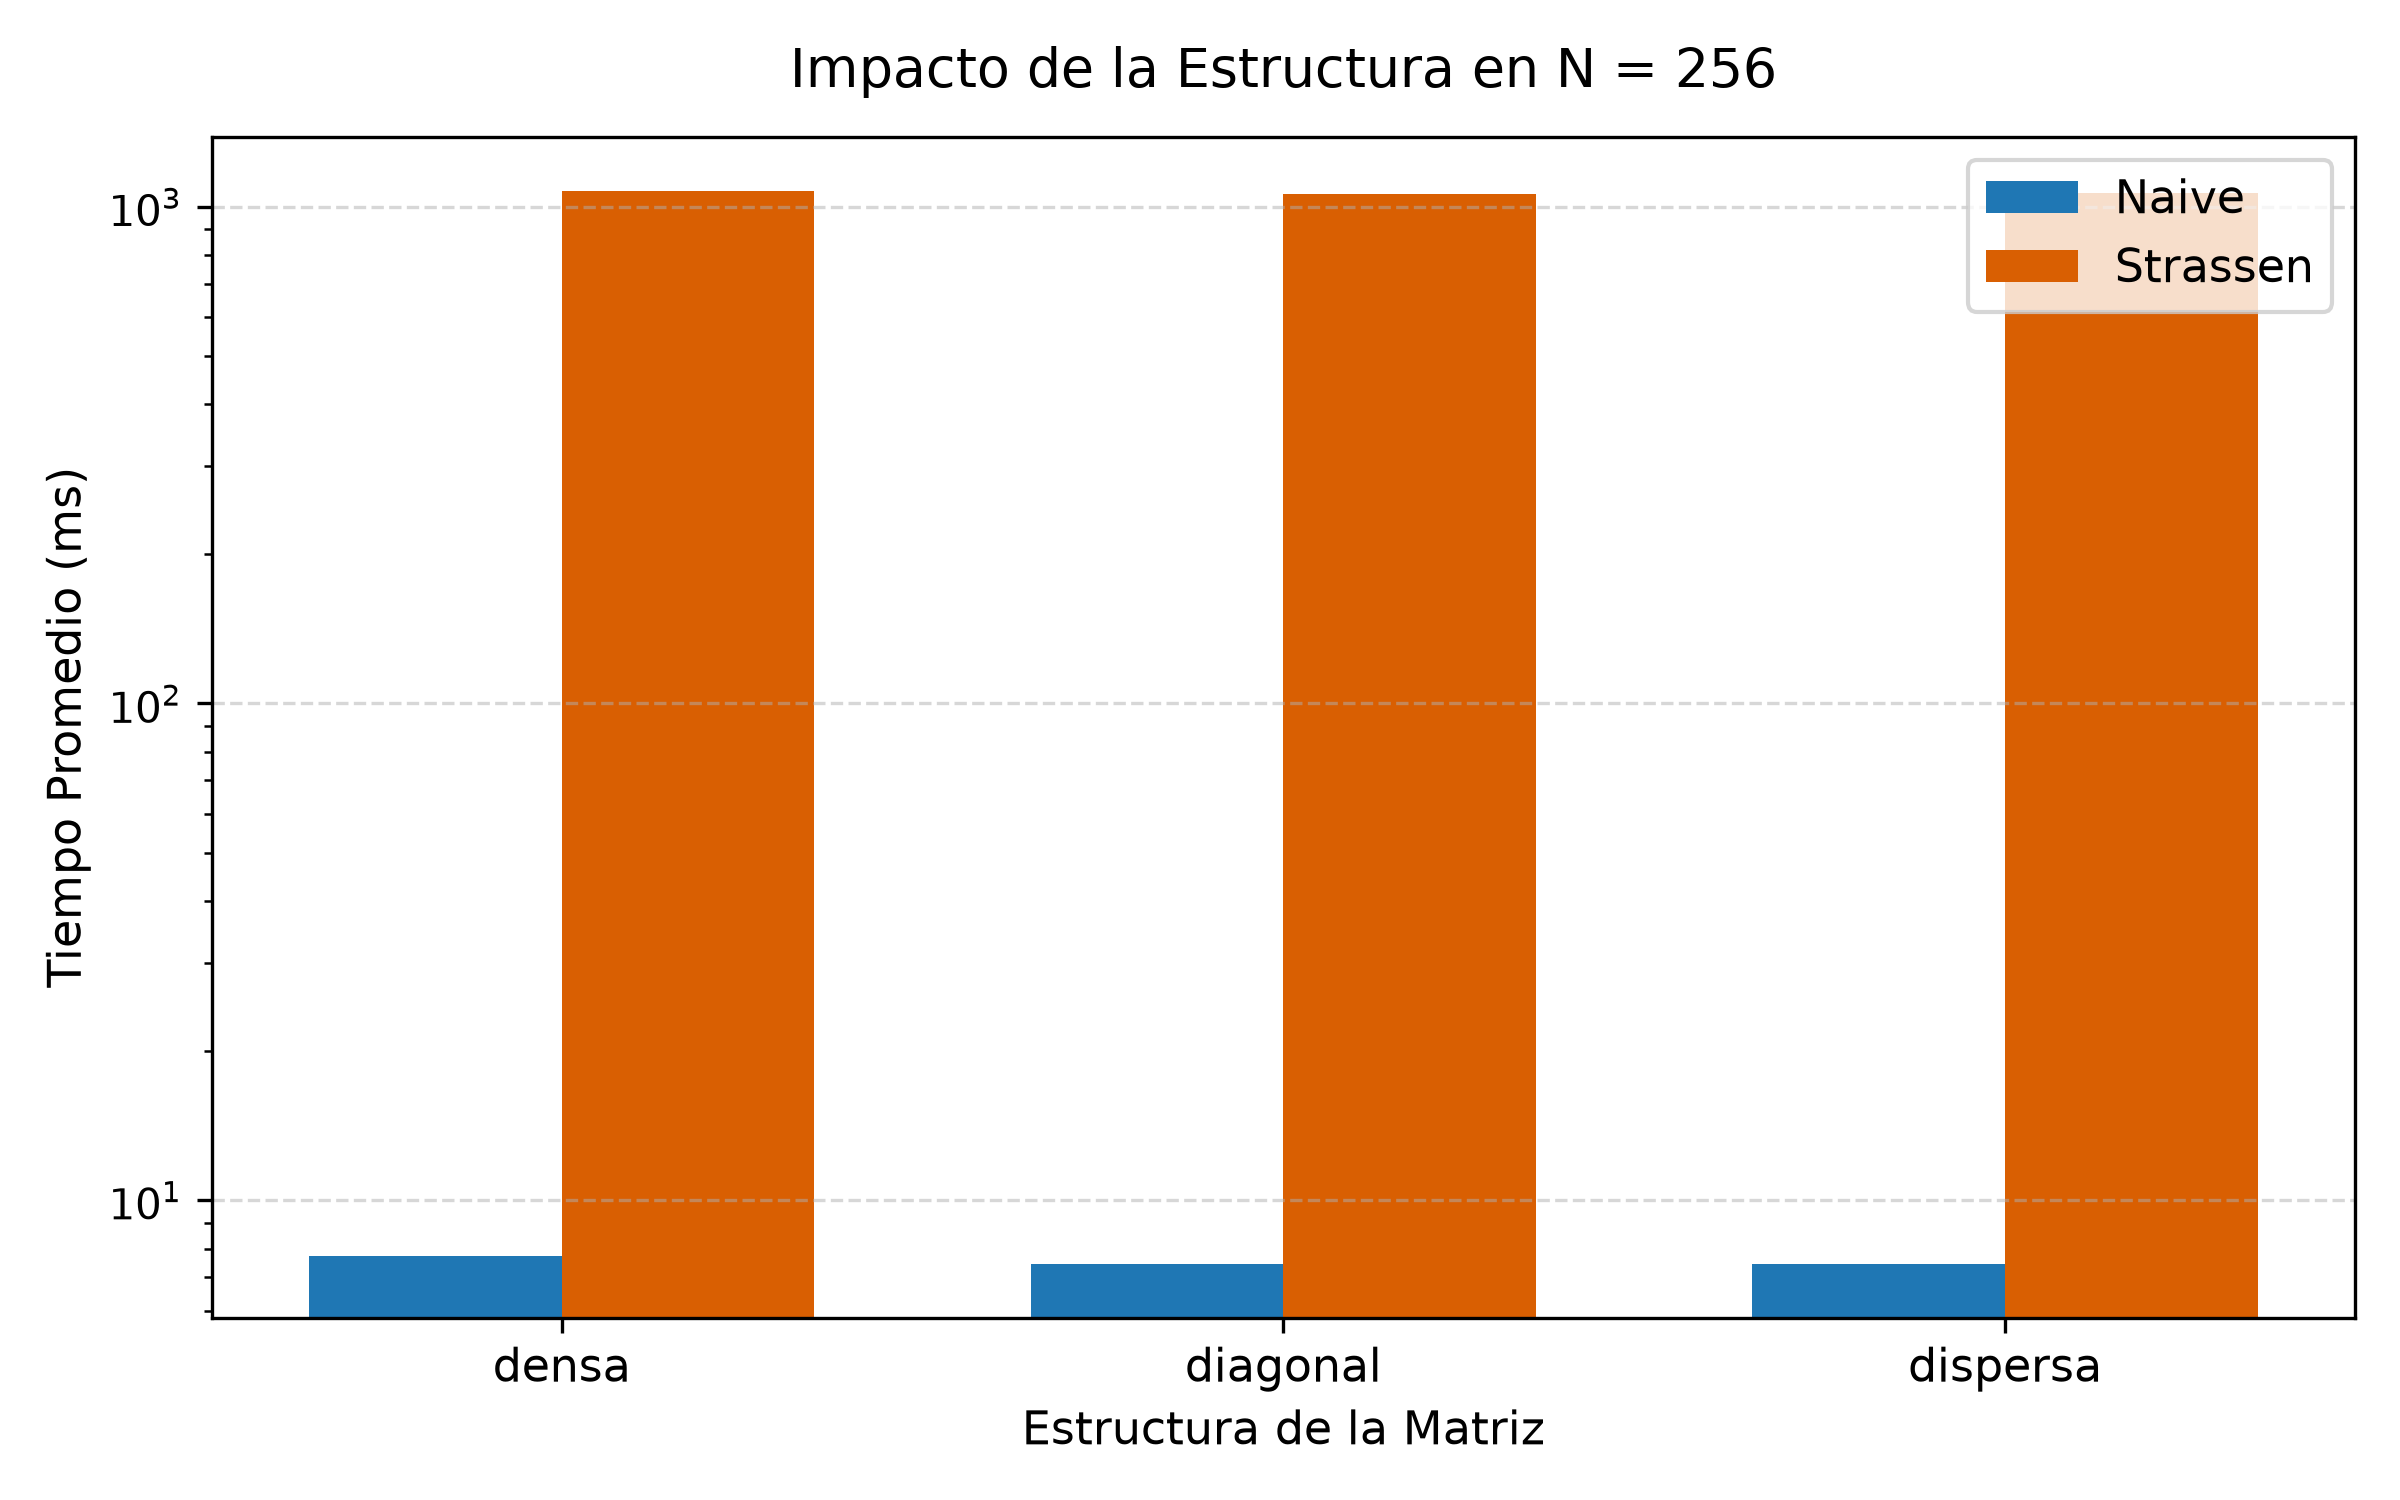
\includegraphics[width=\textwidth]{figures/impacto_tipo_matrices.png}
        \caption{Estructura interna.}
    \end{minipage}\hfill
    \begin{minipage}{0.48\textwidth}
        \centering
        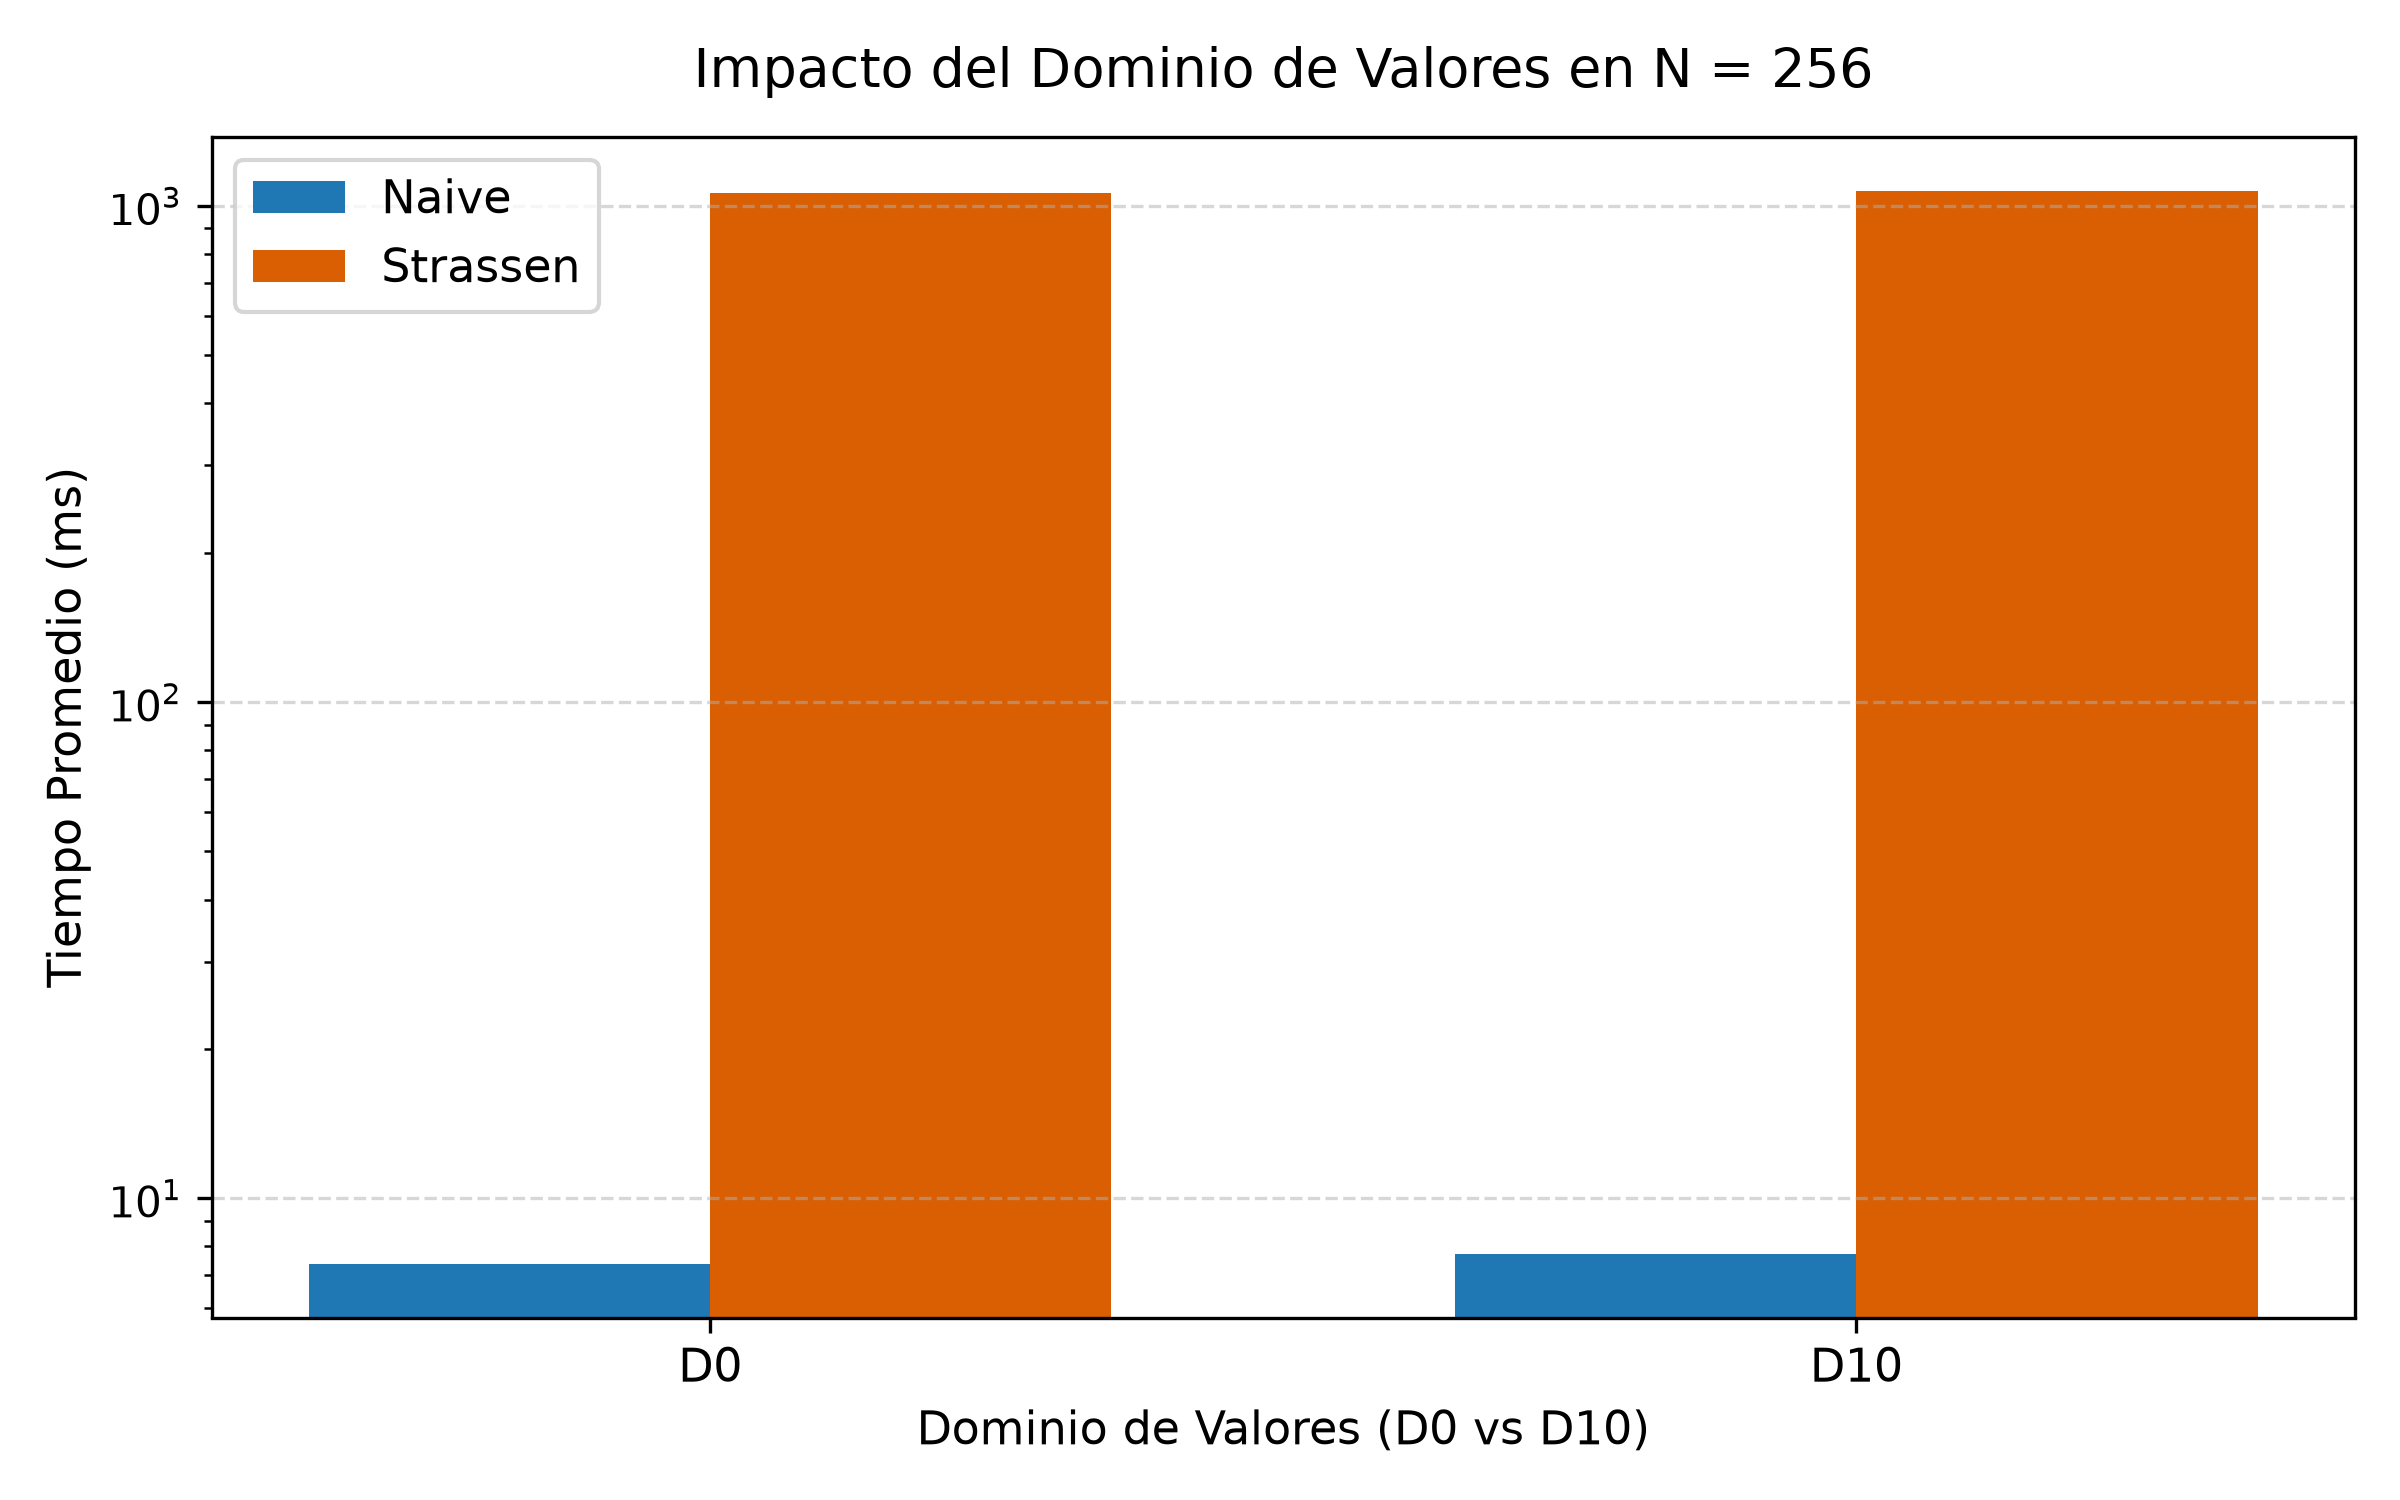
\includegraphics[width=\textwidth]{figures/impacto_dominio_matrices.png}
        \caption{Dominio numérico.}
    \end{minipage}
\end{figure}